\documentclass[a4paper,twoside,DIV15,BCOR12mm]{scrbook}
\usepackage{info}
\usepackage{makeidx}
\usepackage{clrscode}
\usepackage{graphicx}
\usepackage[all]{xy}

\lecturer{Prof. Dr. Müller-Quade}
\semester{Sommersemester 2012}
\scriptstate{unknown}

\author{Die Mitarbeiter von \url{http://mitschriebwiki.nomeata.de/}}
\title{Sicherheit}
\makeindex

\begin{document}
\maketitle

\graphicspath{{./graphics/}}

\renewcommand{\thechapter}{\Roman{chapter}}
%\chapter{Inhaltsverzeichnis}
\addcontentsline{toc}{chapter}{Inhaltsverzeichnis}
\tableofcontents


\chapter{Über dieses Skriptum}
Dies ist ein erweiterter Mitschrieb der Vorlesung \glqq Sicherheit\grqq\ von Herrn Prof. Müller-Quade im
Sommersemester 2012 am Karlsruher Institut für Technologie (KIT).
%Die Mitschriebe der Vorlesung werden mit ausdrücklicher Genehmigung von Herrn Calmet hier veröffentlicht,
%Herr Calmet ist für den Inhalt nicht verantwortlich.

\section{Wer}
Mitgeschrieben in der Vorlesung hat Sabine Oechsner.

\section{Wo}
Alle Kapitel inklusive \LaTeX-Quellen können unter \url{http://mitschriebwiki.nomeata.de} abgerufen werden.
Dort ist ein \emph{Wiki} eingerichtet und von Joachim Breitner um die \LaTeX-Funktionen erweitert.
Das heißt, jeder kann Fehler nachbessern und sich an der Entwicklung
beteiligen. Auf Wunsch ist auch ein Zugang über \emph{Subversion} möglich.


%\renewcommand{\thechapter}{\arabic{chapter}}
%\renewcommand{\chaptername}{§}
%\setcounter{chapter}{0}

%\author{Joachim Breitner, Felix Brandt, Lars Volker}

\chapter{Einleitung}

\section{Was ist Sicherheit?}

\subsubsection{Was soll geschützt werden?}
	\begin{itemize}
		\item Geheimnisse
		\item Daten/Wissen
		\item Dienste/Ressourcen/Infrastruktur
		\item Kommunikation
		\item Ansehen
		\item Rechte (informelle Selbstbestimmung)/Souveränität
		\item Hardware, Maschinen, (Versorgungs)Anlagen
		\item Vermögen, Besitz
		\item Urheberschaft/-recht
		\item Gesundheit/Leben
	\end{itemize}
	
\subsubsection{Vor wem?}
	\begin{itemize}
		\item einzelne (Gelegenheits)Kriminelle
		\item Laien/"Kinder", unerfahrene Benutzer
		\item Spionage, Geheimdienste
		\item organisierte Kriminalität
		\item Saboteure
		\item interessengesteuerte, "nicht-böswillige" Organisationen (Staat, Firmen)
		\item interne Angreifer (Bekannte, Verwandte, Mitarbeiter)
		\item Trojaner
		\item Vandalismus (Skript-Kiddies)
		\item private Feinde/Konkurrenten
	\end{itemize}
	
\subsubsection{Wie?}
	\begin{itemize}
		\item Obscurity, Steganographie
		\item Kryptographie (Verschlüsselung, Signaturen)
		\item physikalische Sicherheit (Bunker, Tresor)
		\item Security Awareness (Mitarbeiterschulung)
		\item Policies, vorgeschriebene Abläufe
		\item Honey Pots, Intrusion Detection
	\end{itemize}
	ganzheitliche Sicherheit (Vermeidung von Schwachstellen):
	\begin{itemize}
		\item Angriffe auf Algorithmenebene (Verschlüsselung brechen, Signatur fälschen)
		\item Angriffe auf Protokollebene (z.B. Replay-, Man-in-the-Middle-Attacken)
		\item Angriffe auf Implementierungsebene (z.B. Bugs ausnutzen, Overflows, Injections)
		\item Angriffe aus Betriebsumgebung (z.B. Power Analysis, Timingattacken)
		\item Angriffe über "externe Komponenten" (z.B. Social Engineering, Phishing)
	\end{itemize}
	
\section{Wichtigste Sicherheitsziele}
	\begin{itemize}
		\item Confidentiality (Schutz vor unbefugten Lesezugriffen)
		\item Integrity (Schutz vor unbefugten Schreibzugriffen (Veränderung/Verfälschung)
		\item Availability (Möglichkeit, Ressourcen/Dienste in der vorgesehenen Form zu nutzen)
	\end{itemize}
	
\section{Praxisprobleme}
	\begin{itemize}
		\item Abwägung Kosten/Nutzen
		\item gesetzliche Regelungen
		\item ethische/soziale Probleme
		\item Grunddilemma unterschiedlicher Begriffe und Definitionen
		\item Snake Oil (z.B. Enigma, Quantenkryptographie + One-Time-Pad)
	\end{itemize}
	
%%%%%%%%%%%%%%% Symmetrische Verschlüsselung %%%%%%%%%%%%%%%%%	
	
\chapter{Symmetrische Verschlüsselung}

\fixme{Definition vernachlässigbare Funktion, S. 4}

\section{Stromchiffren}

\begin{figure}[htb]
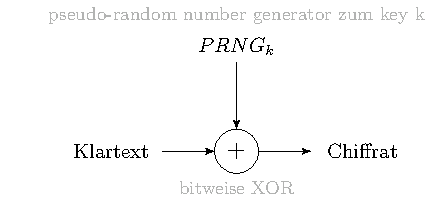
\includegraphics[scale=1]{stromchiffre.pdf}
\end{figure}

\subsection{Anforderungen}
	\begin{itemize}
		\item PRNG muss effizient berechenbar sein
		\item Pseudozufall ununterscheidbar von echtem Zufall\\ (formal: gegeben Orakel $\mathcal{O}_{ideal}$, welches echten Zufall ausgibt, und $\mathcal{O}_{real}$, welches ${PRNG}_k$ mit geheimem Schlüssel $k$ implementiert, gilt für alle (Polynomialzeit)Angreifer $\mathcal{A}$: $\left| Pr\lbrack \mathcal{A}^{\mathcal{O}_{ideal}} \rightarrow 0 \rbrack - Pr\lbrack \mathcal{A}^{\mathcal{O}_{real}} \rightarrow 0 \rbrack \right|$ ist vernachlässigbar in $\left| k \right|$).
	\end{itemize}
	
\section{Blockchiffren}

\subsection{Definition}

Seien $k$ ein Schlüssel aus dem Schlüsselraum $\mathcal{K}$, $A$ und $B$ sind Ein- bzw. Ausgabealphabete und $n$ und $m$ die zugehörigen Blocklängen. Eine Blockchiffre ist eine Familie von injektiven Abbildungen $\{ f_k \colon A^n \rightarrow B^m \}_{k \in \mathcal{K}}$. \\

\fixme{Bild Blockchiffre, S. 4}

\subsection{Anforderungen}

\begin{itemize}
	\item gegeben ein Orakel $\mathcal{O}_{ideal}$, welches eine zufällige Injektion $A^n \rightarrow B^m$ implementiert, und $\mathcal{O}_{real}$, welches $f_k$ mit geheimem Schlüssel $k$ implementiert, gilt für alle (Polynomialzeit)Angreifer $\mathcal{A}$: $\left| Pr\lbrack \mathcal{A}^{\mathcal{O}_{ideal}} \rightarrow 0 \rbrack - Pr\lbrack \mathcal{A}^{\mathcal{O}_{real}} \rightarrow 0 \rbrack \right|$ ist vernachlässigbar in $\left| k \right|$.
	\item gegeben $k$, müssen $f_k$ und $f_k^{-1}$ effizient berechenbar sein
\end{itemize}

\subsection{Beispiel: DES (Data Encryption Standard)}

\fixme{Bild DES, S. 5}

\subsubsection{Eigenschaften}

\begin{itemize}
	\item bis heute strukturell ungebrochen
	\item aber: Schlüssel zu kurz (Brute-Force-Attacken sind heute praktikabel)
\end{itemize}

$\rightarrow$ Abhilfe: 3DES (Chiffrat $= {DES}_{k_3}({DES}^{-1}_{k_2}({DES}_{k_1}(Nachricht)))$)\\
$\rightarrow$ Warum nicht 2DES? Antwort: Meet-in-the-Middle-Attacken

\subsubsection{Meet-in-the-Middle (gegen 2DES):}

\fixme{Bild Meet in the Middle, S. 6}\\

Known-Plaintext-Angriff, gegeben ein Klartext-Chiffrat-Paar $(M, C)$:

\begin{enumerate}
	\item Vorwärts-Schritt: Tabelliere $({DES}_k(M), k)$ für alle Schlüssel $k \in { \{ 0, 1\} }^{56}$.
	\item Sortiere die Tabelle.
	\item Rückwärts-Schritt: Für jedes $k \in { \{ 0, 1\} }^{56}$ berechne $({DES}_k(C)$ und suche Tabelleneintrag mittels binärer Suche.
\end{enumerate}

\paragraph{Aufwand:} $\approx 56 \cdot 2^{56}$ für das binäre Sortieren, $\approx 2^{56}$ für die binäre Suche, insgesamt also nur $\approx 56$ mal mehr Aufwand als bei DES

\subsection{Beispiel: Rijndael/AES (Advanced Encryption Standard)}

\begin{itemize}
	\item 128 bit Blocklänge
	\item 3 Varianten:
		\begin{itemize}
			\item 128, 192, 256 bit Schlüssel
			\item 10, 12, 14 Runden
		\end{itemize}
	\item Darstellung von State und Rundenschlüssel als $4 \times 4$-Byte-Matrix
	\item Ablauf einer Runde in 4 Schritten: \fixme{Bild AES, S. 7}
	\item Bestimmen der Rundenschlüssel:
		\begin{itemize}
			\item teile Schlüssel in 4-Byte-Worte
			\item berechen $W\lbrack i \rbrack := W\lbrack i-4 \rbrack \oplus W\lbrack i-1 \rbrack$ und ab und zu Byteinvertierungen
		\end{itemize}
	\item mögliche Schwäche: AES lässt sich als geschlossene algebraische Gleichung schreiben und ist damit theoretisch mathematisch brechbar
\end{itemize}

\subsection{Betriebsmodi}

\subsubsection{ECB (Electronic Codebook Mode)}

\fixme{Bild ECB, S. 8}\\

Nachteile:

\begin{itemize}
	\item gleiche Klartextblöcke werden auf gleiche Chiffratblöcke abgebildet
	\item Angreifer kann Blöcke vertauschen, löschen, duplizieren
\end{itemize}

Vorteile:

\begin{itemize}
	\item Übertragungsfehler (Bitflips) auf den betroffenen Block begrenzt\footnote{aber: betrifft den ganzen Block, da Verschlüsselung jedes einzelnen Bits im Block von jedem Bit im Block abhängig}
	\item perfekt parallelisierbar (zum Ver- und Entschlüsseln der Blöcke ist jeweils nur der Schlüssel nötig)
	\item verschlüsselte Datenspeicher blockweise bearbeitbar
\end{itemize}

\subsubsection{CBC (Cipher Block Chaining)}

\fixme{Bild CBC, S. 8}\\

Vorteile:

\begin{itemize}
	\item Nachteile von ECB beseitigt
	\item Enschlüsselung selbstsynchronisierend (Klartextblock wird nur aus den letzten beiden Chiffratblöcken berechnet) $\rightarrow$ wahlfreier Lesezugriff
\end{itemize}

Nachteile:

\begin{itemize}
	\item geringer Bandbreitenverlust, da Initialisierungsvektor übertragen werden muss
	\item Fehler breiten sich auf einen weiteren Block aus
\end{itemize}

\subsubsection{OFB (Output Feedback Mode)}

\fixme{Bild OFB, S. 9}\\

Vorteile:

\begin{itemize}
	\item Entschlüsselung muss nicht effizient sein
	\item keine Fehlerübertragung bei Bitflips
	\item Pseudozufallsstrom vorberechenbar
\end{itemize}

Nachteile:

\begin{itemize}
	\item gleicher Initialisierungsvektor bewirkt: $c_1 \oplus c_2 = m_1 \oplus m_2$
	\item nicht robust gegen Verlorengehen ganzer Blöcke
	\item Angreifer kann gezielt Klartextbits kippen
\end{itemize}

\subsubsection{CTR (Counter Mode)}

\fixme{Bild CTR, S. 9}\\

Nachteile:

\begin{itemize}
	\item wie OFB
\end{itemize}

Vorteile (wie OFB und ECB):

\begin{itemize}	
	\item gut parallelisierbar
	\item Pseudozufallsstrom vorberechenbar
	\item Fehlerfortpflanzung auf Blöcke begrenzt
	\item wahlfreier Zugriff auf verschlüsselten Speicher
	\item muss nicht invertierbar sein
\end{itemize}

%%%%%%%%%%%%%%%% Hashfunktionen %%%%%%%%%%%%%%%%%%%%

\chapter{Hashfunktionen}

(hier immer krytographische)

\section{Anwendungen}

\begin{itemize}
	\item Passwortdateien
	\item Time Stamping
	\item Digitale Signaturen (s. \ref{digitale_signaturen})
	\item RSA-ES-OAEP (s. \ref{rsa-es-oaep})
\end{itemize}

\section{Eigenschaften}

einer Hashfunktion $h \colon {\{ 0, 1 \}}^* \rightarrow {\{ 0, 1 \}}^k$:

\begin{itemize}
	\item Einwegfunktion\footnote{die Annahme der Existenz von Einwegfunktionen ist eine stärkere Annahme als $P \neq NP$! $\rightarrow$ Hashfunktionen sind eine noch stärkere Annahme}
	\item preimage resistant: gegeben $x \in {\{ 0, 1 \}}^k$ ist es schwierig, ein $m$ zu finden mit $h(m) = x$
	\item collision resistant: es ist schwierig, $m$ und $m'$, $m \neq m'$, zu finden mit $h(m) = h(m')$
	\item die Ausgabelänge von Hashfunktionen sollte mindestens 160 bit sein (wg. Meet-in-the-Middle-Angriff)
\end{itemize}

\section{Merkle-Damg\r{a}rd-Konstruktion}

gegeben: eine Kompressionsfunktion $f \colon {\{ 0, 1 \}}^{2k} \rightarrow {\{ 0, 1 \}}^k$ (Kandidat: Blockchiffre)\\

\fixme{Bild Merkle-Damgard-Konstruktion, S. 10}\\

Die Sicherheit der so entstandenen Hashfunktion hängt nur von der Sicherheit von $f$ ab. Aber: eine gegebene Kollision lässt sich verlängern.

\section{Das Random Oracle Model}

Manchmal stellt man sich Hashfunktionen vor wie echt zufällige \glqq Orakel\grqq\ . Beweise im Random Oracle Model sind trotzdem nur Heuristiken, da ein Angriff die innere Struktur der Hashfunktion ausnutzen kann.

\section{Der Angriff von Wang}

Der Angriff von Wang findet Kollisionen von MD5 zu gegebenem Initialisierungsvektor. Diese wirken wie zufällig.

\paragraph{Problem (Beispiel Postscript):}

\begin{itemize}
	\item gegeben: Dokumente $P$ und $Q$ und eine Kollision $h(S) = h(R)$
	\item hashe \glqq if\grqq\
	\item nimm dies als Initialisierungsvektor: Kollision $h(\text{if}\ S) = h(\text{if}\ R)$
	\item MD5 ist eine Merkle-Damg\r{a}rd-Konstruktion $\rightarrow$ Erweitern der Kollision zu
		\begin{itemize}
			\item $\text{if}\ S=S\ \text{then display}\ P\ \text{else}\ Q$
			\item $\text{if}\ R=S\ \text{then display}\ P\ \text{else}\ Q$
		\end{itemize}
	\item Ergebnis: zwei Dokumente mit gleichem Hash, aber unterschiedlicher Inhalt wird angezeigt ($P$ oder $Q$)
\end{itemize}

Daher gibt es zur Zeit einen neuen Wettbewerb SHA3.

\section{Symmetrische Authentifikation (MAC - Message Authentification Code)} \label{mac}

Ein MAC ist eine Abbildung ${MAC} \colon {\{ 0, 1 \}}^* \times {\{ 0, 1 \}}^{k}\rightarrow {\{ 0, 1 \}}^k$.

\paragraph{Sicherheitsbegriff:} ein Angreifer $\mathcal{A}$ mit Zugriff auf ein Orakel, das gültige MACs ausrechnet, darf keinen gültigen MAC mit zugehöriger Nachricht finden können, ohne das Orakel nach dieser Nachricht gefragt zu haben.

\begin{itemize}
	\item Vorschlag 1: $h(key \| m)$ $\rightarrow$ funktioniert nicht \fixme{warum?}
	\item Vorschlag 2: $h(m \| key)$ $\rightarrow$ funktioniert nicht \fixme{warum?}
	\item HMAC: $h((key \oplus o\_pad) \| h((key \oplus i\_pad) \| m))$
\end{itemize}

\fixme{Bild HMAC, S. 12}

%%%%%%%%%%%%%%%% Schlüsselaustausch %%%%%%%%%%%%%%%%

\chapter{Schlüsselaustausch}

Verschlüsselung und Authentifikation benötigen einen gemeinsamen geheimen Schlüssel:

\section{3-Pass}

(Schlüssel-/Nachrichtenaustausch mit mittelalterlichen Mitteln)\\

\fixme{Bild 3-Pass oben, S. 14}\\

Problem: Man-in-the-Middle-Angriff möglich (Bote befestigt eigenes Schloss, statt Kiste zu Bob zu bringen) $\rightarrow$ Abhilfe: z.B. schwer fälschbare Siegel auf dem Schloss

\subsubsection{modernere Idee:}

Nachrichtentransfer über authentifizierten, aber nicht abhörsicheren Kanals mittels OTP (One-Time-Pad):\\

\fixme{Bild 3-Pass unten, S. 14}\\

\paragraph{Problem:} das funktioniert so nicht, da $$(M \oplus OTP\_Alice) \oplus (M \oplus OTP\_Alice \oplus OTP\_Bob) = OTP\_Bob$$

\section{Wide-Mouth-Frog}

\fixme{Bild Wide-Mouth-Frog, S. 15}\\

Probleme:

\begin{itemize}
	\item benötigt vertrauenswürdige Zentrale
	\item Zentrale zuständig für Verbindungsaufbau zu Bob $\rightarrow$ DoS-Attacke möglich
	\item Alice benötigt guten Zufallsgenerator
\end{itemize}

\section{Kerberos}

\fixme{Bild Kerberos, S. 15}\\

\begin{enumerate}
	\item $(\text{alice}, \text{bob})$
	\item $({Enc}_{k_{AZ}}(T_Z, L, K_{AB}, \text{bob}), {Enc}_{k_{BZ}}(T_Z, L, K_{AB}, \text{alice}))$
	\item $({Enc}_{k_{AB}}(\text{alice}, T_A), {Enc}_{k_{BZ}}(T_Z, L, K_{AB}, \text{alice}))$
	\item ${Enc}_{k_{AB}}(T_A + 1)$
\end{enumerate}

Probleme:

\begin{itemize}
	\item benötigt synchrone Uhren
	\item Chiffre muss non-malleable\footnote{aus einem Chiffrat darf sich kein anderes gültiges berechnen lassen} sein, sonst evtl. $Enc_{T_{AB}}(T_A + 1)$ aus $Enc_{T_{AB}}(T_A)$ berechenbar $\rightarrow$ Confidentiality $\nRightarrow$ Non-Malleability!
\end{itemize}

Die ältere Variante Needham-Schroeder hatte noch keine Zeitstempel, sondern Zufallszahlen. $\rightarrow$ Replay-Attacken möglich (z.B. Alice ist eine Kamera und der Angreifer spielt alte Aufnahmen wieder ein)

\section{Merkle Puzzle}

Alice wählt zufällig $k$ Paare von Schlüssel und zufälliger Schlüsselnummer und verschlüsselt die Paare mit einer symmetrischen Chiffre mit immer neuem Schlüssel. Sie schickt alles an Bob zusammen mit genügend Hinweisen, sodass Bob jedes der verschlüsselten Paare \glqq brechen\grqq\ kann. Bob entschlüsselt eines der Paare und antwortet Alice mit der Schlüsselnummer des von ihm gebrochenen Paares und die beiden kennen nun einen gemeinsamen Schlüssel.\\ Der \glqq Vorteil\grqq\ von Alice und Bob gegenüber einem Lauscher ist leider nur gering (quadratisch).

\section{Diffie-Hellman-Schlüsselaustausch (DH)}

Seien eine (öffentlich bekannte) Gruppe $G$ sowie ein Erzeuger $g$ dieser Gruppe gegeben\footnote{hier muss der diskrete Logarithmus schwierig zu berechnen sein!} (z.B. $\mathbb{F}_p^\times, p \in \mathbb{P}$ oder eine Gruppe auf einer Elliptischen Kurve):\\

\fixme{Bild DH, S. 16}\\

Diffie-Hellman ist (beweisbar) sicher relativ zur Decisional-Diffie-Hellman-Annahme.

\subsection{Decisional-Diffie-Hellman-Annahme}

Asymptotisch ist es nicht in Polynomialzeit möglich, folgende Verteilungen zu unterscheiden: $(g, g^a, g^b, g^{ab})$ und $(g, g^a, g^b, g^c)$ mit $a, b, z$ zufällig.

\subsection{Man-in-the-Middle-Angriff}

\fixme{Bild Man-in-the-Middle-Angriff, S. 17}\\

Verhindern von Man-in-the-Middle-Angriffen:

\begin{itemize}
	\item symmetrische Authentifikation (s. \ref{mac}) mit einem Langzeitgeheimnis
	\item digitale Signaturen (s. \ref{digitale_signaturen})
\end{itemize}

%%%%%%%%%%%%%%% Public-Key-Kryptographie %%%%%%%%%%%%%%%%

\chapter{Public-Key-Kryptographie}

Ein bisschen zu den mathematischen Grundlagen findet sich im Kapitel \ref{mathe}.

\section{Definition}

\fixme{Definition}

\section{Sicherheitsbegriff: IND-CCA2-Sicherheit}

\fixme{Definition}

\section{Beispiel: Elgamal}

Seien $G$ eine Gruppe mit Erzeuger $g$, $a$ zufällig.

\begin{itemize}
	\item öffentlicher Schlüssel von Alice: $g^a$
	\item geheimer Schlüssel von Alice: $a$
	\item Verschlüsseln einer Nachricht $m$: 
		\begin{itemize}
			\item wähle $b$ zufällig und berechne $g^b$
			\item verschicke $(g^b, g^{ab} \oplus m)$\footnote{oder $(g^b, g^{ab} \cdot m)$}
		\end{itemize}
	\item Entschlüsseln eines Chiffrats $c$: mithilfe von $a$
\end{itemize}

\section{Beispiel: RSA}

Sei $N \in \mathbb{N}$ mit $N = p \cdot q$ für $p$, $q$ prim. Wähle ein zu $\varphi(N) = (p-1)(q-1)$ teilerfremdes $e$ mit $1 < e < \varphi(N)$ und berechne $d := e^{-1} \mod \varphi(N)$.

\begin{itemize}
	\item öffentlicher Schlüssel: $(e, N)$
	\item geheimer Schlüssel: $(d, N)$
	\item Verschlüsseln einer Nachricht $m$: $c = m^e \mod N$
	\item Entschlüsseln eines Chiffrats $c$: $m = c^d \mod N$
\end{itemize}

\subsection{Die RSA-Funktion}

Die Funktion $x \mapsto x^e \mod N$ wird auch als RSA-Funktion bezeichnet. Sie ist eine Permutation auf $(\mathbb{Z}/N\mathbb{Z})^\times$.

\subsection{Textbook-RSA}

Das oben beschriebene Verfahren wird oft auch als Textbook-RSA bezeichnet.  Es ist nicht sicher, da gleiche Klartexte immer auf gleiche Chiffrate abgebildet werden.

\subsubsection{Beispiel Auktionsangriff}

\fixme{Bild Auktionsangriff, S. 20}

\subsection{RSA-ES-OAEP} \label{rsa-es-oaep}

Hier kommt bei der Berechnung des Chiffrats eine Zufallszahl $r$ ins Spiel: $c = ((m + h(r)) \| (h(m + h(r)) +r))^e$. Zur Entschlüsselung bilde zunächst $c^d$. Dann hashe den ersten Teil der Nachricht, um durch Addieren des Hashs zum zweiten Teil der Nachricht den Zufall zu bekommen. Nun kann die eigentliche Nachricht berechnet werden.

\subsubsection{Sicherheit}

RSA-ES-OAEP ist beweisbar sicher im Random Oracle Model: Ein Angreifer, der das IND-CCA2-Spiel gewinnt, kann benutzt werden, um die RSA-Funktion zu invertieren.


%%%%%%%%%%%%%%%%%% Digitale Signaturen %%%%%%%%%%%%%%%%

\chapter{Digitale Signaturen} \label{digitale_signaturen}

\section{Begriffe}

\begin{itemize}	
	\item Authentizität (d.h. einer Person eindeutig zugeordnet)
	\item Integrität (d.h. unverändert)
	\item Unabstreitbarkeit (non repudiation)
	\item Praktikabilität (d.h. kurz im Vergleich zum Dokument)
\end{itemize}

\section{Beispiel: Signieren mit RSA (anschaulich)}

Man \glqq entschlüsselt\grqq\ das Dokument, als wäre es ein Chiffrat. Dies kann nur der Besitzer des Secret Keys. Prüfen kann aber jeder, der den Private Key kennt: \glqq Verschlüsseln\grqq\ der Signatur ergibt die Nachricht.\\ Signatur zu $m$ wäre dann $m^d \mod N = \sigma$ und überprüfen via $\sigma^e \mod N \stackrel{?}{=} m$.\\

So ist das aber noch nicht sicher:

\begin{enumerate}
	\item zu zufälligem $r$ wirkt $r$ wie eine gültige Signatur von $r^e \mod N$
	\item $\sigma_1 \cdot \sigma_2 \mod N$ ist eine gültige Signatur, da $(m_1^d) \cdot (m_2^d) = (m_1 \cdot m_2)^d \mod N$
\end{enumerate}

Abhilfe: Hash-then-Sign (beweisbar sicher im Random Oracle Model)

\section{Definition Signatur}

\fixme{Definition Signatur, S. 25}

\section{Sicherheitsbegriff: EUF-CMA}

\section{Beispiel: Elgamal-Signaturen}

Sei $G$ eine Gruppe mit Erzeuger $g$ ($G = \mathbb{F}_p$ für $p$ prim)\footnote{Rechnen: bei Gruppenelementen $\mod{p}$, im Exponenten $\mod{(p-1)}$}. Wähle $x$ zufällig.

\begin{itemize}
	\item öffentlicher Schlüssel (Verifikationsschlüssel): $vk = g^x$
	\item signing key: $sk = x$
\end{itemize}

Signatur \glqq naiv\grqq\ :

\begin{itemize}
	\item signieren: $M \equiv ax \mod{(p-1)}$ $\rightarrow$ Signatur: a
	\item prüfen: $g^M \equiv g^{ax} \equiv {vk}^a \mod{(p-1)}$
	\item aber: $x \equiv Ma^{-1} \mod{(p-1)}$ und jeder kann nun den $sk$ ausrechnen
\end{itemize}

deshalb:

\begin{itemize}
	\item signer Bob wählt $k$ zufällig mit $ggT(k, p-1) = 1$
	\item $ a :\equiv g^k \mod{p}$
	\item berechne $b$ mit $m \equiv x \cdot a + k \cdot b \mod{(p-1)}$
	\item Signatur zu $m$ ist $(a,b)$
	\item Prüfen der Signatur: $g^m \equiv g^{xa+kb} \equiv g^{xa} \cdot g^{kb} \equiv {vk}^a \cdot a^b \mod{p}$
\end{itemize}

\subsection{Probleme}

\begin{enumerate}
	\item niemals ein $k$ zweimal verwenden $\rightarrow$ mit $m_1 = xa +kb_1$ und $m_2 = xa + kb_2$ lässt sich $x$ berechnen
	\item es ist möglich, gültige Signaturen zu (unsinnigen) Nachrichten zu generieren $\rightarrow$ Lösung: hash-then-sign
\end{enumerate}

\section{Beispiel: DSA (Digital Signature Algorithm)}

$g \in \mathbb{F}_p^\times$ erzeuge eine multiplikative Gruppe der Ordnung $q \in \mathbb{P}$, ($q | p-1$).

\begin{itemize}
	\item $sk = x$
	\item $vk = g^x$
\end{itemize}

Signieren:

\begin{itemize}
	\item wähle $k \in \{0, dotsc, q-1\}$ zufällig
	\item berechne $r :\equiv g^k (\mod{p}) \mod{q}$
	\item berechne $s$ mit $h(m) \equiv k\cdot s - x \cdot r \mod{q}$
	\item dann ist $(r,s)$ eine Signatur zu $m$
\end{itemize}

Prüfen: $r \equiv (g^{s^{-1}h(m)} vk^{s^-1}r \mod{p}) \mod{q}$

\section{Beispiel: One-Time-Signaturen (aus Hashfunktionen)}
		
$sk$ besteht aus zufälligen Strings $\in {\{0,1 \}}^k$

$$r_1^0\ r_2^0\ r_3^0\ \ldots\ r_k^0$$
$$r_1^1\ r_2^1\ r_3^1\ \ldots\ r_k^1$$

$vk$ ist

$$h(r_1^0)\ h(r_2^0)\ h(r_3^0)\ \ldots\ h(r_k^0)$$
$$h(r_1^1)\ h(r_2^1)\ h(r_3^1)\ \ldots\ h(r_k^1)$$

Beispielsignatur zu $01\ldots1$: $r_1^0\ r_2^1\ \ldots\ r_k^1$\\

One time signatures darf man nur einmal verwenden! Alternativ kann man einen doppelt so langen $vk$ benutzen: Signiere die Nachricht und einen neuen public key (der wieder zwei Nachrichten signieren kann). Zum Verifizieren benötigt man eine Kette signierter $vk$s, die zum ursprünglichen public key führen. Wenn die Nachrichten länger als $k$ bit sind, verwendet man hash-then-sign.

\section{Ist EUF-CMA genug?}

\subsection{Key Substitution Attacks}

\begin{itemize}
	\item Alice hat $vk$ und signiert $m$ mit $\sigma$
	\item Bob wählt (böse) einen $vk'$, sodass seine Signatur zu $m$ exakt $\sigma$ ist
\end{itemize}

\subsubsection{Beispiel (RSA)}

\begin{enumerate}
	\item Wähle $\bar p$ und $\bar q$ so, dass $\bar p -1$ und $\bar q - 1$ in kleine Primfaktoren zerfallen und $\sigma$ und $h(m)$ $\mathbb{F}_{\bar p}^\times$ und $\mathbb{F}_{\bar q}^\times$ generieren.
	\item Pohlig-Hellman-Algorithmus löst den dlog $\mod{\bar p}$ und $\mod{\bar q}$.
	\item Berechne $x_1$, $x_2$, sodass $\sigma^{x^1} \equiv h(m) \mod{\bar p}$ und $\sigma^{x^2} \equiv h(m) \mod{\bar q}$.
	\item Ist $ggT(\bar p -1, \bar q - 1) = 2$, so gibt es ein eindeutiges $\bar e < \varphi(\bar p \bar q)$ mit $\bar e \equiv x_1 \mod{\bar p - 1}$ und $\bar e \equiv x_2 \mod{\bar q - 1}$ (Chinesischer Restsatz).
	\item Gib $(\bar n = \bar p \cdot \bar q, \bar e)$ als $vk$ aus.
\end{enumerate}

Dann gilt: $\sigma^{\bar e} \equiv h(m) \mod{\bar n}$, d.h. Signatur gilt, weil $\sigma^{\bar e} \equiv h(m) \mod{\bar p}$ und $\sigma^{\bar e} \equiv h(m) \mod{\bar q}$.

\subsubsection{Lösungen}

\begin{itemize}
	\item DSA ist sicher gehen (starke) Key Substitution
	\item $vk$ immer mitsignieren
\end{itemize}

\subsection{Subliminal Channel}

Gut Simmons hat gemerkt, dass Signaturen Nachrichten enthalten können (subliminal channels). 

\subsubsection{Beispiel:}

RSA-PSS signiert eine spezielle Kodierung:\\

\fixme{Bild RSA-PSS, S. 29}

%%%%%%%%%%%%%%%% Key Management %%%%%%%%%%%%%%%%

\chapter{Key Management}

oder Wie benutzt man Public-Key-Kryptographie?

\section{PKI (Public-Key-Infrastruktur)}

\subsection{\glqq Definition\grqq}

Ein digitales Zertifikat ordnet einem öffentlichen Schlüssel eindeutig einen Inhaber zu.\\ Eine Public-Key-Infrastruktur ist die Gesamtheit der organisatorischen Maßnahmen, die für eine vertrauenswürdige Ausgabe und Verifikation von Zertifikaten notwendig ist.\\

Aufgaben einer PKI sind z.B. die Ausstellung, Verteilung, Prüfung und der Widerruf digitaler Zertifikate. (Impliziert dies, dass der Inhaber seinen eigenen secret key kennt?)

\section{Beispiel: X.509-Zertifikat}

(die folgende Liste ist nicht vollständig)

\begin{enumerate}
	\item Versionsnummer $\in \{1,2,3\}$, je nachdem, welche erweiterten Elemente vorhanden sind
	\item Seriennummer, wird von Certification Authority (CA) gewählt und sollte pro CA eindeutig sein
	\item Signaturalgorithmus und Parameter
	\item Distinguished Name (DN) des Ausstellers
	\item Gültigkeitsdauer
	\item Distinguished Name des Inhabers
	\item Public-Key-Informationen: Algorithmus, Parameter, public key
	\item Erweiterungen
	\item Signatur auf 1.-8.
\end{enumerate}

\section{Certificate Revocation}

mittels Certificate Revocation Lists (CRL) (Listen einer CA, die widerrufene Zertifikate enthalten)\\

Diese enthalten ein Ausstellungsdatum und das Datum der nächsten geplanten CRL. Zertifikate bleiben auf der CRL, bis sie abgelaufen sind. (Genauer: Online Certificate Status Protocols)

\section{Web of Trust}

$\mathrel{\widehat{=}}$ sozialem Netzwerk von \glqq Mini-CAs\grqq.

\begin{itemize}
	\item Key-Signing-Partys zum Signieren
	\item Jeder kann selbst festlegen, welchen anderen Usern er vertraut.
\end{itemize}

Im Einzelfall unsicherer (schlecht geschützte CAs), aber Angriffe skalieren nicht so.

\section{TLS (Transport Layer Security)}

\begin{itemize}
	\item Standard im Internet
	\item Nachfolger von SSL-Protokollen
\end{itemize}

\subsection{Ablauf}

\fixme{Bild TLS, S. 31}

Jeder kann eine key-renegotiation beantragen und das Protokoll startet dann neu.

\subsection{Besonderheiten}

\begin{itemize}
	\item Schutz gegen Downgrade (kein Versionswechsel während Protokollablauf)
	\item die Nachricht \glqq Finish\grqq\ enthält einen Hash über alle bisherigen Protokollnachrichten der Session
	\item die verwendete pseudozufällige Funktion teilt den Input in zwei Hälften, hasht mit MD5 und SHA1 und XORs die Ergebnisse $\rightarrow$ das bleibt sicher, auch wenn beispielsweise MD5 Schwächen zeigt (\glqq Robust Combiner\grqq)
\end{itemize}
		
\section{Key Renegotiation Attack}

auf TLS

\subsection{Ziel} 

Client und Server sollen sich in unterschiedlichen Anwendungskontexten befinden, was der Angreifer ausnutzen kann (z.B. Client will Passwort senden, Server will nächste Nachricht an Adresse XY weiterleiten)

\subsection{Ablauf}

\fixme{Bild Key Renegotiation Attack, S. 32}
	
%%%%%%%%%%%%%%%%% Netzwerksicherheit %%%%%%%%%%%%55	
	
\chapter{Netzwerksicherheit}

\section{CIA-Paradigma}

\begin{itemize}
	\item Confidentiality
	\item Integrity
	\item Availability
\end{itemize}

(das ist noch keine vollständige Spezifikation, aber ein \glqq Template\grqq)

\section{Sicherheitsbegriff}

\begin{itemize}
	\item Vertraulichkeit
	\item Integrität
	\item Data origin authentification
	\item Peer entity authentification
	\item Non repudiation (Nichtabstreitbarkeit)
		\begin{itemize}
			\item proof of origin
			\item proof of delivery/submission
			\item proof of receipt
		\end{itemize}
\end{itemize}

\section{Das ISO/OSI-Referenzmodell}

\begin{tabular}{ll}
7 & Anwendungsschicht\\
6 & Präsentationsschicht\\
5 & Sitzungsschicht\\
4 & Transportschicht\\
3 & Netzwerkschicht\\
2 & Verbindungsschicht\\
1 & Physikalische Schicht
\end{tabular}

Sicherheitseigenschaften sollen/können durch darunterliegende Schichten nicht gefährdet werden. (Ausnahme: Anonymität)

\section{IPsec}

Protokollsuite, die Authentifikation und Verschlüsselung von IP-Paketen sowie entity authentification und key exchange erlaubt (bringt Sicherheit schon auf Ebene 3).\\

Schneier, Ferguson: \glqq IPsec was a great disappointment to us.\grqq\\

Im Wesentlichen: zu komplex.

\section{Bedrohungen für Rechner in Netzwerken}

(Liste nicht vollständig)

\begin{itemize}
	\item Belauschen, Unterdrücken, Verfälschen von Daten
	\item Portscan (automatisches Scannen von Schwachstellen)
	\item Fingerprinting (z.B. Ermitteln der OS-Version)
	\item Angriffe auf das Routing
	\item Schwachstellen in anderen Protokollen (z.B. DNS)
	\item Denial-of-Service-Attacken (DoS)
	\item Angriffe von innen
	\item Viren, Würmer, Trojaner
	\item Backdoors
\end{itemize}

\section{Schutzmaßnahmen}

\subsection{Firewalls}

\begin{itemize}
	\item Paketfilter (Aussortieren nach Adressen/Diensten)
	\item Stateful Inspection (berücksichtigt zusätzliche Verbindungsinformationen)
\end{itemize}

\fixme{Bilder Firewall, S. 34}\\

Firewalls sind eine Präventivmaßnahme, die ergänzt werden sollten durch Monitoring.

\subsection{Monitoring}

Intrusion Detection Systems

\subsection{Honeypots}

\subsection{Datendiode}

Datenversand nur in eine Richtung möglich\\

\fixme{Bild Datendiode, S. 35}

%%%%%%%%%%%%%% Zugriffskontrolle %%%%%%%%%%%%%%%%%%%%%

\chapter{Zugriffskontrolle}

(wirkt ein bisschen altmodisch, heute usage control)

\section{Bell-LaPadula-Modell}

Das Bell-LaPadula-Modell ist ein statisches Zugriffskontrollmodell. Oberstes Schutzziel: Confidentiality

\subsection{Definition}

\begin{itemize}
	\item Subjektmenge $\mathcal{S}$
	\item Objektmenge $\mathcal{O}$
	\item Menge von Zugriffsoperationen $\mathcal{A} = \{ read, write, append, execute \}$
	\item Menge $\mathcal{L}$ von Security Levels mit einer partiellen Ordnung $\leq$
\end{itemize}

Dabei implizieren $write$-Rechte die $read$-Rechte. (Beispiel: unclassified $\leq$ confidential $\leq$ secret $\leq$ top secret)\\

Im Bell-LaPadula-Modell ist der Systemzustand ein Element aus $\mathcal{B} \times \mathcal{M} \times \mathcal{F}$, wobei:

\begin{itemize}
	\item $\mathcal{B} = \mathcal{P}(\mathcal{S} \times \mathcal{O} \times \mathcal{A})$ aktuelle Zugriffe beschreibt (wer hat Zugriff auf was mit welcher Zugriffsart)
	\item $\mathcal{M}$ die Menge der Zugriffskontrollmatrizen (ACM) bezüglich der Subjekte in $\mathcal{S}$ und der Objekte in $\mathcal{O}$ ist. Die Elemente von $\mathcal{M}$ haben die Form $M = (M_{so})_{s \in \mathcal{S}, o \in \mathcal{O}}$ mit $M_{so} \subseteq \mathcal{A}$ für alle $s \in \mathcal{S}, o \in \mathcal{O}$.
	\item $\mathcal{F}$ Dreitupel aus Funktionen enthält, den sog. Security Level Assignments. Hier gilt $\mathcal{F} \subseteq \mathcal{L}^\mathcal{S} \times \mathcal{L}^\mathcal{S} \times \mathcal{L}^\mathcal{O}$. Ein Dreitupel $(f_s, f_c, f_o)$ hat dabei folgende Form und Bedeutung:
		\begin{itemize}
			\item $f_s \colon \mathcal{S} \rightarrow \mathcal{L}$ gibt für jedes $s' \in \mathcal{S}$ den maximalen Sicherheitslevel an
			\item $f_c \colon \mathcal{S} \rightarrow \mathcal{L}$ gibt den gegenwärtigen (current) Sicherheitslevel an
			\item $f_o \colon \mathcal{O} \rightarrow \mathcal{L}$ gibt für jedes $o' \in \mathcal{O}$ den Sicherheitslevel an
		\end{itemize}
		Dabei gilt: $f_c$ muss von $f_s$ dominiert werden: $\forall s' \in \mathcal{S} \colon f_c(s') \leq f_s(s')$.
\end{itemize}

Ein Systemzustand heißt sicher, wenn er die folgenden drei Eigenschaften erfüllt:

\begin{itemize}
	\item Simple Security Property (ss-Eigenschaft):\\ ein Zustand $(b,M,f)$ genügt der ss-Eigenschaft, falls $\forall (s',o',a') \in b$ mit $a \in \{read, write\}$ gilt: $f_s(s') \geq f_o(o')$ (\glqq no read up\grqq)
	\item Star Property (*-Eigenschaft):\\ ein Zustand (b,M,f) erfüllt die *-Eigenschaft, falls $\forall (s',o',a') \in b$ mit $a \in \{append, write\}$ gilt: $f_c(s') \leq f_o(o')$ (\glqq no write down\grqq)\\ Weiterhin, falls ein $(s', o',a) \in b$ mit $a \in \{append, write\}$ und ein $(\hat s, \hat o, \hat a) \in b$ mit $s' = \hat s$ und $\hat a \in \{read, write\}$ existiert, dann muss $f_o(\hat o) \leq f_o(o')$ gelten. (\glqq Kein Nachrichtenfluss von high level object zu low level object.\grqq)
	\item Discretionary Security Property (ds-Eigenschaft):\\ ein Zustand $(b,M,f)$ erfüllt die ds-Eigenschaft, falls $\forall (s',o',a) \in b$ stehts $a \in M_{s'o'}$ gilt
\end{itemize}

\subsection{Basic Security Theorem}

Werden ausgehend von einem sicheren Initialzustand nur sichere Übergänge durchgeführt, so erhält man einen sicheren Systemzustand.

\subsection{Nachteile}

Leider sammelt sich im Bell-LaPadula-Modell Information \glqq oben\grqq, ein Deklassifizieren ist nicht möglich. In der Praxis werden etwa \glqq trusted subjects\grqq\ eingeführt, um ein Deklassifizieren von Daten zu erlauben.\\

Weitere Nachteile:

\begin{itemize}
	\item Integrität der Daten wird nicht mitbetrachtet (niedrigstufige user/Prozesse können evtl. höher eingestufte Objekte verändern)
	\item keine Forderung an die ACM, etwa darf allen $s \in \mathcal{S}$ alle Rechte gegeben werden
	\item verdeckte Kanäle, z.B. die (Nicht)Existenz von Dateien, bleiben unberücksichtigt
\end{itemize}

\subsection{Vorteile}

\begin{itemize}
	\item handhabbar
	\item formal (d.h. für Beweise geeignet)
\end{itemize}

\section{Chinese-Wall-Modell}

Zugriffsrechte hängen von der Vergangenheit ab $\rightarrow$ z.B. kein Informationsfluss zwischen konkurrierenden Firmen (z.B. bei Unternehmensberatung)

\subsection{Definition}

\begin{itemize}
	\item Menge $\mathcal{C}$ von Firmen
	\item Objektmenge $\mathcal{O}$ (jedes Objekt gehört einer Firma)
	\item Subjektmenge $\mathcal{S}$ (die Berater)
	\item Funktion $y \colon \mathcal{O} \rightarrow \mathcal{C}$, welche jedem Objekt die zugehörige Firma zuordnet
	\item Funktion $x \colon \mathcal{O} \rightarrow \mathcal{P}(\mathcal{C})$, welche jedem Objekt eine conflict-of-interest-Klasse zuordnet
\end{itemize}

Die Sicherheitsmarke (security label) eines Objekts $o \in \mathcal{O}$ ist das Tupel $(x(o), y(o))$. Im Falle $x(o) = \emptyset$ spricht man von \glqq sanitized information\grqq.\\

Eine Matrix $M$ enthält Informationen über Zugriffe $M = (M_{so})_{s \in \mathcal{S}, o \in \mathcal{O}}$ mit
$$M_{so} = 	\begin{cases}
				true,  & \text{falls }s\text{ Zugriff auf }o\text{ hatte,}\\
				false, & \text{sonst.}
			\end{cases}$$
			
Der Initialzustand ist $M = (false)_{s \in \mathcal{S}, o \in \mathcal{O}}$.

\subsection{Eigenschaften}

\begin{itemize}
	\item Simple Security Property (ss-Eigenschaft):\\ $s \in \mathcal{S}$ erhält Zugriff auf $o \in \mathcal{O}$ nur, falls $\forall o' \in \mathcal{O}$ mit $M_{so'} = true$ gilt: $y(o) = y(o')$ oder $y(o) \notin x(o')$.
	\item Star Property (*-Eigenschaft):\\ ein $s \in \mathcal{S}$ erhält Schreibzugriff auf ein Objekt $o \in \mathcal{O}$ nur, falls $s$ aktuell keinen Lesezugriff auf $o' \in \mathcal{O}$ hat mit $y(o) \neq y(o')$ oder $x(o') = \emptyset$. (Die *-Eigenschaft verhindert die Weitergabe von Daten über Dritte.)
\end{itemize}

%%%%%%%%%%% Zero Knowledge %%%%%%%%%%%%%%%%%

\chapter{Zero Knowledge}

Idee: Wir wollen (interaktiv) beweisen, dass wir ein Geheimnis kennen, ohne das Geheimnis selbst zu verraten. 

\section{Eigenschaften:} 

\begin{itemize}
	\item Korrektheit: Ein Beweiser, der das Geheimnis nicht kennt, soll einen Prüfer nur mit vernachlässigbarer Wahrscheinlichkeit davon überzeugen können, es zu kennen.
	\item Zero Knowledge: Für jeden Prüfer gibt es einen Simulator, der einen Mitschrieb der Beweiskommunikation selbst erzeugen kann, ohne den Beweis zu kennen.
\end{itemize}

\section{Beispiel: Graph-Isomorphismus}

\subsection{Ablauf}

\begin{itemize}
	\item allen bekannt: zwei Graphen $G_1$ und $G_2$
	\item Geheimnis des Beweisers: ein Graph-Isomorphismus zwischen $G_1$ und $G_2$
	\item der Beweiser erzeugt einen weiteren zufälligen Graphen, der isomorph zu $G_1$ und $G_2$ ist, und gibt ihn dem Prüfer
	\item der Prüfer fordert den Isomorphismus vom neuen Graphen zu einem der beiden Graphen $G_i$
	\item der Beweiser gibt den Isomorphismus bekannt
	\item das Spiel wird häufig wiederholt
\end{itemize}

\subsection{Eigenschaften}

\begin{itemize}
	\item kennt der Beweiser das Geheimnis, so kann er dem Prüfer immer den geforderten Isomorphismus angeben
	\item Korrektheit: kennt er ihn nicht, kann er nur einen der beiden Isomorphismen angeben (den, mit dem er den neuen Graphen erzeugt hat), und wird bei häufigem Wiederholen erwischt
	\item Zero Knowledge: weiß der Beweiser vorher, welchen Isomorphismus der Prüfer sehen will, so bereitet er genau diesen vor
\end{itemize}

\section{Beispiel: Graph-3-Färbbarkeit}

Mit Graph-3-Färbbarkeit wird die Frage bezeichnet, ob zu einem gegebenen Graphen eine Knotenfärbung mit 3 Farben existiert, sodass direkt verbundene Knoten immer ungleiche Farben haben. Graph-3-Färbbarkeit ist ein NP-vollständiges Problem.

\subsection{Ablauf}

\begin{itemize}
	\item allen bekannt: ein Graph $G$
	\item Geheimnis des Beweisers: eine 3-Färbung von $G$
	\item der Beweiser benennt die Farben zufällig um (dabei bleibt die Färbung eine 3-Färbung)
	\item der Beweiser verschlüsselt alle Knoten und zeigt dies dem Prüfer
	\item der Prüfer wählt eine Kante
	\item der Beweiser entschlüsselt die zugehörigen Knoten
	\item dieses Spiel wird häufig wiederholt (mit immer neuer Vertauschung der drei Farben, damit der Prüfer das Geheimnis nicht lernen kann)
\end{itemize}

\subsection{Eigenschaften}

\begin{itemize}
	\item Korrektheit: gibt es keine 3-Färbung, so sind immer irgendwo zwei Farben gleich und der Beweiser wird bei häufigem Wiederholen erwischt
	\item Zero Knowledge: weiß der Beweiser vorher, welche Kante gefragt wird, verschlüsselt er dort zwei zufällige, verschiedene Farben
\end{itemize}

%%%%%%%%%%%%%% Authentifikation %%%%%%%%%%%55

\chapter{Authentifikation}

\section{Definition}

Authentifizierung bindet eine Identität an ein Subjekt.

\section{Ansätze}

\begin{itemize}
	\item Entität weiß etwas (Kennwort)
	\item Entität ist etwas (Biometrie)
	\item Entität hat etwas (Chipkarte)
	\item Entität kann etwas (Captcha)
	\item Entität befindet sich an einem bestimmten Ort
\end{itemize}

\section{Komponenten}

\begin{itemize}
	\item Menge $A$ der Authentifizierungsinformation\\ (Information, mit der Identität bewiesen wird)
	\item Menge $C$ der Komplementärinformationen\\ (was das System speichert, um Authentifizierung zu validieren)
	\item Menge $\mathcal{F} \in C^A$ der Komplementierungsfunktionen\\ (leitet aus gegebenem $a \in A$ das entsprechende $c \in C$ ab)
	\item Menge $L \subseteq {\{ true, false \}}^{A \times C}$ der Authentifikationsfunktionen\\ (verifiziert Identifikation)
	\item Menge $S$ der Auswahlfunktionen\\ (zum Anlegen, Ändern, Entfernen von Entitäten und entsprechenden Daten)
\end{itemize}

\section{Typische Anwendung: Kennworte}

\begin{itemize}
	\item 1. Ansatz: System speichert Kennworte explizit\\ $\rightarrow$ Problem: Diebstahl des Passwordfiles
	\item 2. Ansatz: kryptographische Hashwerte der Kennworte speichern\\ $\rightarrow$ Problem: Offline-Wörterbuchattacke sehr effizient
	\item 3. Ansatz: Saltung (pro Benutzer andere Hashfunktion): $H_s(pw) := H(pw \| s)$
	\item 4. Ansatz: \glqq Remote-Login\grqq\ mit dediziertem Authentifizierungsserver
\end{itemize}

\section{Maßnahmen gegen Offline-Attacken}

\subsection{Wahl guter Kennworte}

\begin{itemize}
	\item vorgegebene Zufallsstrings (werden aufgeschrieben und am Rechner deponiert)
	\item \glqq Key-Crunching\grqq\ $\rightarrow$ Hashing langer Passphrases
	\item Verschleierung aufgeschriebener Kennworte (einfache Transformation)
	\item proaktive Kennwortwahl
	\item zeitliche Variation (ganz gut: ab und zu Kennwort verlängern)
	\item Security Awareness
\end{itemize}

\section{Maßnahmen gegen Online-Attacken}

\begin{itemize}
	\item Backoff $\rightarrow$ nach $n$ Fehleingaben Sperrung für $x_n$ Sekunden
	\item Disconnection $\rightarrow$ nach $n$ Fehleingaben Verbindungstrennung
	\item Jailing $\rightarrow$ begrenzter Zugriff wird trotz Fehleingabe gewährt, oft mit Honeypots kombiniert
\end{itemize}

\section{Beispiel: CAPTCHAs}

automatisch generierte Rätsel, die Maschinen nur sehr schwer lösen können, Menschen dagegen sehr leicht

\section{Raffiniertere Verfahren (Challenge-Response)}

\subsection{Schema} Benutzer hat Geheimnis $s$\\

\fixme{Bild Schema, S. 53}\\

Das Geheimnis $S$ soll nicht aus $c$ und $c(r,s)$ rekonstruierbar ein (selbst bei böswillig gewähltem $c$).

\subsection{Beispiele}

\subsubsection{RSA-Signaturen} Server schickt String, lässt ihn sich signieren $\rightarrow$ in der Praxis manchmal zu aufwändig
\subsubsection{mittels Hashfunktion oder Verschlüsselung} $r(s.c) = h(s,c)$ oder $r(s,c) = Enc_s(c)$ $\rightarrow$ Server muss Geheimnis $S$ kennen
\subsubsection{Zero Knowledge} $\rightarrow$ in der Praxis zu aufwändig
\subsubsection{SPEKE (Simple Password Encrypted Key Exchange)}

Parameter:

	\begin{itemize}	
		\item $p = 2q + 1$, $p,q \in \mathbb{P}$ (\glqq safe prime\grqq)
		\item Hashfunktion $H$
		\item $g = H(Passwort)^2 \mod{p}$ (erzeugt die Gruppe der quadratischen Reste $\mod{p}$)
	\end{itemize}
	
\paragraph{Ablauf:} wie Diffie-Hellman, aber $key := H(g^{ab})$ sowie mit Key Confirmation\\ 

\fixme{Bild Ablauf, S. 53}

\paragraph{möglicher Angriff:} schicke $g^a =1$ oder $g^a$ mit kleiner Ordnung $\rightarrow$ Schlüssel unabhängig von Passwort $\rightarrow$ Lösung: Protokollabbruch, falls $Ord(g^{ab} < q$

%%%%%%%%%%%% Seitenkanalangriffe %%%%%%%%%%%

\chapter{Seitenkanalangriffe}

\fixme{schreib mich ;)}

%%%%%%%%%%%% Implementierungsfehler %%%%%%%%%%%%%

\chapter{Implementierungsfehler}

\section{in Programmen}

\begin{itemize}
	\item Stack/Heap Overflows
	\item Integer Overflows, Signed-Unsigned-Bugs
	\item falsche Unicodebehandlung
	\item Ausnutzen von Race Conditions
	\item \glqq Environment Creep\grqq\ (es war unter anderen Umständen sicher, aber die Umstände haben sich geändert)
	\item Ändern temporärer Dateien
\end{itemize}

\section{in Webanwendungen}

\begin{itemize}
	\item SQL injection
	\item XSS (Cross Site Scripting)
	\item GIFAR (Datei entspricht gif- und jar-Standard)
	\item Variablenvorbelegung bei PHP
\end{itemize}

\section{Lektion fürs Leben}

\begin{itemize}
	\item Komplexität ist ein Feind der Sicherheit.
	\item Sicherheit komponiert nicht.
\end{itemize}

%%%%%%%%%%%% Sicherheitsbewertung/Zertifizierung %%%%%%%%%%%5

\chapter{Sicherheitsbewertung/Zertifizierung}

Beurteilung durch eine vertrauenswürdige Instanz (bescheinigt Eigenschaften) $\rightarrow$ meist wird allerdings nicht ein Produkt, sondern der Entwicklungsprozess zertifiziert

\section{Gründe für eine Zertifizierung}

\begin{itemize}
	\item gesetzliche Bestimmungen (Datenschutz)
	\item Werbung
	\item überzeugt Nichtexperten
	\item günstigere Versicherung
	\item Vergleich von Produkten \glqq einfacher\grqq
\end{itemize}

\section{Common Criteria (ISO 15408)}

Zertifizierungsstelle in Deutschland: BSI (Bundesamt für Sicherheit in der Informationstechnik)

\begin{itemize}
	\item ToE (Target of Evaluation)
	\item Protection Profile $\rightarrow$ Forderungen an das ToE
		\begin{itemize}
			\item Descriptive Elements:
				\begin{itemize}
					\item worum geht es? (Smartcard, Firewall, ...)
					\item was ist das Problem, das damit gelöst werden soll?
				\end{itemize}
			\item Rationale (Zuordnung zwischen Bedrohungen/Angriffen und Sicherheitseigenschaften):
				\begin{itemize}
					\item welche Betriebsumgebung?/welches Einsatzszenario?
					\item welche Bedrohungen/Angriffe?
					\item welche Sicherheitseigenschaften?
				\end{itemize}
			\item Functional Requirements: funktionale Spezifikation des ToE
			\item Evaluation Assurance Requirements:
				\begin{itemize}
					\item wie/was wird evaluiert? (es gibt umfangreiche Beispielkataloge)
					\item wie intensiv wird evaluiert?
				\end{itemize}
		\end{itemize}
\end{itemize}

\subsection{Evaluation Insurance Levels}

numerische Bewertung der Prüfstrenge

\begin{itemize}
	\item EAL 1: funktional getestet
	\item EAL 2: strukturell getestet
	\item EAL 3: methodisch getestet und überprüft
	\item EAL 4: methodisch entwickelt, getestet und durchgesehen
	\item EAL 5: semiformal entworfen und getestet
	\item EAL 6: semiformal verifizierter Entwurf und getestet
	\item EAL 7: formal verifizierter Entwurf und getestet
\end{itemize}

%%%%%%%%%%%% Data Base Privacy %%%%%%%%%%%%%%%%

\chapter{Data Base Privacy}

\section{k-Anonymität}

\fixme{Bild k-Anonymität, S. 57}\\

für jede Kombination der QI in der Datenbank gibt es k Zeilen mit dieser Kombination (z.B. durch Vergröbern der QIs)

\subsection{Kritik}

\begin{enumerate}
	\item nur das Ergebnis wird beurteilt, nicht der Prozess (Seitenkanäle)
	\item komponiert nicht
	\item Homogenitätsattacke
\end{enumerate}

\section{Differential Privacy}

Datenbanken sind Mengen von Tupeln aus $\mathbb{R}^d$. Ein Release Mechanism nimmer eine Datenbank und liefert eine Zahl aus $\mathbb{R}$. Zwei Datenbanken haben \glqq Hammingabstand\grqq\ 1, wenn sie sich nur in einem Tupel unterscheiden. Für zwei beliebige Datenbanken (aus einem gegebenen Universum) mit Hammingabstand 1 soll der Release sich höchstens um $\epsilon$ unterscheiden: \glqq $\epsilon$-differentially private\grqq.\\

Methode für Release: Verrauschen

%%%%%%%%%%%%%% Secure Function Evaluation %%%%%%%%

\chapter{Secure Function Evaluation}

\section{Beispiel: Datingproblem}

Alice und Bob haben ein Rendezvous, vermittelt von Datingagentur. Wie entscheiden, ob man sich wieder trifft? (peinlich, falls nur einer will...)

\subsection{Lösung: Secure AND}

jeder gibt geheimes Bit ein und lernt nur das AND-Ergebnis

\paragraph{Realisierung}

\begin{itemize}
	\item Input Alice: Bit $a$
	\item Input Bob: Bit $b$
\end{itemize}

\begin{enumerate}
	\item Alice generiert Signaturkey $x$ und sendet Verifikationskey $y$ an Bob
	\item Alice generiert $(e,d,N)$ und sendet $(e,N)$ an Bob
	\item Bob wählt $s$, berechnet $r_b:= Enc(s)$, $r_{1-b} := N-b$ und sendet $(r_0, r_1)$ an Alice
	\item Alice sendet $c_0 = sign(0) + Dec(r_0)$ und $c_1 = sign(a + Dec(r_1))$ an Bob
	\item Bob berechnet $sign(ab) = c_b - s$ und teilt Alice das Ergebnis mit
\end{enumerate}

Wofür Signieren? $\rightarrow$ sonst kann Bob immer $b = 1$ wählen und Alice über das Ergebnis belügen (und $a$ herausfinden).\\ Wenn Alice nur eine Signatur richtig berechnet, hängt es von $b$ ab, ob das Protokoll regulär durchgeht. $\rightarrow$ Lösung: ZK-Beweis\\

Achtung: Signatur darf keinen Subliminal Channel haben

\section{allgemeine Secure Function Evaluation}

\subsection{Baustein: \glqq oblivious transfer\grqq\ (OT)}

\begin{itemize}
	\item Input Alice: Strings $a_0$, $a_1$
	\item Input Bob: Bit $b$
	\item Output Alice: nichts
	\item Output Bob: $a_b$
	\item Alice lernt nichts über $b$
	\item Bob lernt nichts über $a_0$ oder nichts über $a_1$
\end{itemize}

\subsection{Realisierung}

\begin{enumerate}
	\item Alice generiert $(e,d,N)$ und sendet $(e,N)$ an Bob
	\item Bob wählt $s$, berechnet $r_b = Enc(s)$, $r_{1-b} = N-b$ und sendet $(r_0, r_1)$ an Alice
	\item Alice sendet $c_0 = a_0 + Dec(r_0)$ und $c_1 = a_1 + Dec(r_1)$ an Bob
	\item Bob berechnet $a_b = c_b - s$
\end{enumerate}

\subsection{Realisierung mit Funktion $f$}

hier ist der Input von Bob ein String $b$

\begin{itemize}
	\item Alice stellt Wertetabelle $F$ für $f(a, \cdot)$ auf
	\item Für jedes Bit von $b$ sendet Alice zwei Zufallswerte $k_0$, $k_1$ via OT an Bob; es bezeichne $(k_0^i, k_1^i)$ das zu $b_i$ gehörige Tupel. Bob lernt jeweils $k_{b_i}^i$.
	\item Alice verschlüsselt $F$ zeilenweise; die zu $b$ zugehörige Zeile von F ist verschlüsselt mit dem XOR über $k_{b_i}^i$.
	\item Alice sendet die verschlüsselten Zeilen an Bob.
	\item Bob kann genau die zu $b$ gehörige Zeile entschlüsseln und lernt $f(a,b)$.
\end{itemize}

\paragraph{Probleme:}

\begin{enumerate}
	\item Wie sicherstellen, dass Alice die richtige Funktion $f$ codiert? $\rightarrow$ ZK-Beweis
	\item Wie sicherstellen, dass Bob über das Ergebnis nicht lügen kann? $\rightarrow$ Signaturen
	\item Tabelle $F$ ist exponentiell groß in $\left|b\right|$ $\rightarrow$ \glqq Yao's Garbled Circuits\grqq
\end{enumerate}

\subsection{Yao's Garbled Circuits}

\begin{itemize}
	\item Zerlege Schaltkreise von $f$ in einzelne Gatter und wende obiges Protokoll auf jedes einzelne Gatter an.
	\item Bob darf keine Zwischenergebnisse lernen, deshalb werden Gatterergebnisse direkt durch entsprechende Schlüssel ersetzt, statt die Schlüssel via OT zu übertragen (natürlich nur für Gatter, deren Ergebnis nicht Teil der Ausgabe des Schaltkreises ist).
	\item Bob weiß nicht mehr, welche Zeile einer Tabelle für ein Gatter innerhalb des Schaltkreises er entschlüsseln muss; deshalb werden verschlüsselte Nullstrings an jede Tabellenzeile angehängt, Bob entschlüsselt immer die ganze Tabelle und verwirft \glqq falsche\grqq\ Zeilen.
	\item Bob kann noch aus der Position der \glqq richtigen\grqq\ Zeile einers Gatters die Eingangsbelegung erkennen; daher werden jeweils die Zeilen einer Tabelle zufällig permutiert.
\end{itemize}
		
%%%%%%%%%%%%%% Mathematisches %%%%%%%%%%%%%%%%%%%%

%\chapter{Mathematisches} \label{mathe}

\section{Gruppen}

\subsection{Definition}

Eine Gruppe ist eine Menge $G$ mit einer Verkn�pfung $*$, sodass gilt:

\begin{itemize}
	\item die Verkn�pfung ist assoziativ
	\item es gibt ein Element $e_G$, sodass f�r alle $g \in G$ $g * e_G = e_G * g =g$ gilt (neutrales Element
	\item f�r alle $g \in G$ gibt es ein $g^{-1}$, sodass $g * g^{-1} = e_G$ gilt
\end{itemize}

Die Ordnung einer Gruppe ist die Anzahl ihrer Elemente.

\subsection{Satz von Lagrange}

Sei $G$ eine endliche Gruppe, $U \leq G$ eine Untergruppe von G. Dann teilt die Ordnung von $U$ die Ordnung von $G$.\\

Insbesondere erzeugt jedes Element $g \in G$ eine Untergruppe von $G$. Die Ordnung dieser Untergruppe teilt dann nat�rlich wieder die Ordnung von $G$.

\subsection{Kleiner Satz von Fermat}

\subsection{Eulersche $\varphi$-Funktion}

Die Eulersche $\varphi$-Funktion einer nat�rlichen Zahl $N$ ist definiert als die Anzahl der nat�rlichen Zahlen kleiner $N$, die zu $N$ teilerfremd sind: $\varphi(N) = \left|(\mathbb{Z}/N\mathbb{Z})^\times \right| = \left| \{ x \mid x \in \mathbb{N}, x < N, x \not| N \} \right|$

\section{Euklidischer Algorithmus}

\section{Chinesischer Restsatz (f�r $\mathbb{Z}$)}

%\appendix
%\chapter{Satz um Satz (hüpft der Has)}
%\listtheorems{satz,wichtigedefinition}

%\renewcommand{\indexname}{Stichwortverzeichnis}
%\addcontentsline{toc}{chapter}{Stichwortverzeichnis}
%\printindex

%\include{Ana2Credits}

\end{document}
